% !TEX root = ../../main.tex
%

\chapter{Background} \label{chap:background}

Concurrency control is crucial in systems where multiple processes or threads simultaneously access shared resources, such as data structures, tables, or files. 
Effective concurrency control mechanisms employ various synchronization techniques to maintain the safety and consistency of these shared resources. As noted by \citet{DBLP:books/daglib/0030596}, "Synchronization is a set of rules and mechanisms that allows the specification and implementation of sequencing properties on statements issued by the processes so that all the executions of a multiprocess program are correct."

In this chapter, we provide an introduction to multi-granularity locking. We discuss the structure of a hierarchy and the operations that can be performed on hierarchical data structures. We discuss the challenges of hierarchical data structures and the need for specialized locking techniques to manage concurrent access. 



\section{Hierarchical data structures}

Hierarchical data models, rooted in the early days of computer science, play a critical role in the representation and storage of structured information. The inception of hierarchical data can be traced back to the 1960s with the development of the Information Management System (IMS) by IBM \cite{IBMIMS}. IMS was one of the earliest database management systems designed specifically for organizing hierarchical data and was created to manage the complex manufacturing data associated with the Apollo space program. IMS establishes a well-defined parent-child relationship between data entities, a characteristic of hierarchical models \cite{DBLP:books/daglib/0006734}.

Over the decades, hierarchical data structures have remained pertinent, particularly in domains that require nested or tree-like relationships. They are widely utilized in XML data management, file system hierarchies, and organizational charts \cite{DBLP:books/mk/BunemanSA99}. The relevance of hierarchical models has only increased in contemporary big-data contexts, where they are often integrated with other data models, such as graphs, to address the challenges posed by the complexity and interconnectedness of modern data environments.

For instance, hierarchical data models are fundamental in NoSQL databases like Apache HBase, where the efficient storage and rapid retrieval of large-scale, semi-structured data are critical \cite{DBLP:books/daglib/0027893}. The structured nature of hierarchical models aligns well with applications in social networks, content management systems, and cloud-based storage solutions, where understanding and managing data relationships is essential.
Consequently, hierarchical data models remain foundational to modern computing, providing an effective framework for organizing and retrieving complex, nested information.

\subsection{Structure of a hierarchy}
A hierarchy is a tree-like structure with an additional property, such that a vertex can have multiple parents.
Formally, a hierarchy is defined as follows:

\begin{definition}
    A hierarchy is a directed graph H=(V, E, R) and R $\in$ V where
    \begin{itemize}
        \item V is a finite set of vertices.
        \item $E \subset V \times V$ is a set of directed edges where each edge (u, v) represents a parent-child relationship between vertices u (the parent) and v (the child).
        \item R is the designated root of the hierarchy such that there is a path from R to every other vertex in V.
        
    \end{itemize} 
\end{definition}

\subsection{Data in hierarchical data structures}

Hierarchical data structures are used to represent data that has a natural hierarchical relationship. This data is stored in the form of key-value pairs. Each vertex in a hierarchy has a unique identifier, type, and set of attributes. The data stored in the vertices can be of any kind, ranging from simple data types like integers and strings to complex data types like arrays and objects. 

Vertices are connected by edges that represent the relationships between them. These relationships are directional and often labelled. The labels on the edges can be used to represent the type of relationship between the vertices. For example, in a file system, the edges can be labelled as "contains" to represent the relationship between a directory and the files it contains. \cref{fig:hierarchicalDS} shows an example of a hierarchical data structure with data on vertices and edges. In this hierarchy, vertices represent entities of type "Person". Each person has a unique identifier and the amount of food they possess. Person vertices are connected via edges labelled \texttt{:isFriendTo} with a weight representing the strength of the friendship. So, we can infer that \emph{"Asterix is close friends with Obelix and a casual friend with Getafix"}.


\begin{figure}[h]
    \centering
    \captionsetup{justification=centering}
    \includegraphics[width=\textwidth]{figures/HierarchicalDSExample.png}
    \caption{An example of a hierarchical data structure with data on vertices and edges.}
    \label{fig:hierarchicalDS}
\end{figure}




\subsection{Operations in hierarchical data structures}

Hierarchical data structures support various operations that enable querying and modifying the data. These operations are essential for managing data in the vertices and relationships between vertices of the hierarchy. Common operations on hierarchical data structures fall into two categories:

\begin{itemize}

    % \item \textbf{Search and Query:} Searching and querying operations involve locating specific vertices or paths within the hierarchy based on predefined criteria. These operations are essential for retrieving relevant information from the data structure. These operations result in read-only access to the hierarchy. While Data reads focus on vertices, search and query operations focus on relationships between vertices and use the edges to navigate the hierarchy.
    
    \item \textbf{Data read and write:} A data read and write operation involves accessing and/or updating attributes of vertices in a hierarchy. These operations are fundamental for interacting with the data and retrieving information from the structure. One or more vertices are often involved in a single read or write operation, depending on the application's specific requirements. These operations do not alter the topology of the hierarchy.

    \item \textbf{Structural modifications:} Inserting and deleting vertices or edges in a hierarchical structure can alter the observable topology of the hierarchy. These operations are crucial for creating new data and maintaining the integrity of the relationships between vertices. We call such operations \emph{structural modifications}.
    

\end{itemize}

\section{Locking, consistency and performance}
The primary goal of a multi-granularity locking protocol is to find an effective way of locking an entire \emph{sub-graph}. In a hierarchy, each vertex can be locked individually. This can be done to read or write the data on the vertex. However, in many applications, it is sometimes necessary to lock an entire sub-graph to ensure that the data remains consistent. For example, a file system must lock the directory as a whole to ensure that another concurrent thread does not modify the files within the directory.


When write-locked, the requester has exclusive access to a vertex and implicitly to all its descendants. When read locked, a requester has shared access to the vertex and implicitly to all its descendants. Since MGL aims to lock entire sub-graphs, preventing another transaction from acquiring a lock on a vertex that is an ancestor of a locked vertex is essential. Assume a vertex $v$ is locked in write mode. This implicitly locks the entire subtree rooted at $v$ in write mode. If another transaction acquires a lock on an ancestor $a$ of $v$, the sub-graph rooted at $a$, which also contains the sub-graph rooted at $v$, is implicitly locked. This violates the core invariant of MGL, which is to provide isolated sub-graph access to threads. To prevent this, MGL must ensure that another transaction locks no ancestor of a locked vertex. 

An important concern of an application, after correctness, is performance. The performance of a correct locking protocol is determined by the rate at which locks can be granted, i.e., \emph{locking throughput}. A correct application that is slow is often not useful in practice. In database design, this performance is driven by the choice of \emph{lockable units}. A lockable unit is a set of data which should be atomically locked to ensure data consistency. A smaller lockable unit allows for more concurrency and better performance if transactions are simple, i.e., do not access many data items. Complex transactions access several data items and incur significant overhead in acquiring and releasing locks. A larger lockable unit is more efficient in such cases as it reduces this overhead.
On the other hand, to ensure consistency, a larger lockable unit discriminates against transactions that access only a few data items by requiring them to wait. It is, therefore, desirable to vary the size of this lockable unit based on the access requirement of a transaction and have varying sizes of lockable units in the system. This is the motivation behind multi-granularity locking. 

\section{Multi-granularity locking: terminology and concepts}
This section introduces the key concepts and terminology associated with multi-granularity locking (MGL) in hierarchical data structures. These concepts are essential for understanding the challenges and solutions MGL protocols present.
In particular, concepts like "lock grain," which describe the lockable units in hierarchical locking, are critical for understanding the nuances of how concurrency is managed in graph-based data models. While some of these terms are standard in the literature, others are specific to the context of this thesis, reflecting the unique challenges and solutions presented by hierarchical data structures.


\paragraph{Lock target} The lock target refers to a specific vertex or a set of vertices within the hierarchy that a transaction accesses. A transaction may access a single lock target or a set of them. A lock target is defined independently of a locking protocol.  

\paragraph{Lock guard} The lock guard is an entity that serves as the point of synchronization for a given set of lock targets. A thread must acquire the corresponding lock guard to ensure data consistency when accessing a particular target. The lock guard acts as a sentinel, preventing other threads from modifying the protected data until the lock is released. The mapping between a lock target and its corresponding lock guard depends on the locking protocol. We shall see examples of this in \cref{chap:relatedwork}.

\paragraph{Lock grain} Lock grain refers to the scope of implicitly locked data when a lock is acquired on a guard. A lock grain is a lockable unit protected by multi-granularity locks. A grain is rooted at a vertex and includes all descendants of that vertex. This root is designated as the lock guard for the grain.

\paragraph{Granularity} The size of the grain is called its \emph{granularity}, which varies from coarse-grained locks that encompass large portions of the hierarchy (e.g., entire sub-graphs) per lock guard to fine-grained locks that target individual vertices or smaller groups of vertices per lock guard. The choice of lock grain (resp. granularity) directly impacts the level of concurrency and performance in a system. In contrast, fine-grained locks allow for greater parallelism; they can introduce additional complexity in managing locks.

\subsection{Access modes and conflicts}

MGL protocols lock grains in either read or write mode. A read lock on a grain allows other transactions to acquire read locks on the same grain but prevents any transaction from acquiring a write lock. A write lock on a grain prevents any other transaction from acquiring a read or write lock.
Two lock requests are compatible if they can be granted concurrently. MGL determines this compatibility by two conditions: \textbf{mode conflict} and \textbf{grain conflict}. 

A mode conflict is dependent on the semantics of the lock. MGL uses the standard read/write lock semantics. A write lock guarantees lock grain exclusivity and is incompatible with any other lock request. A read lock allows shared access to a grain and is compatible with other read locks but not write locks. Some MGL protocols, like intention locks, further develop this concept by introducing additional modes to indicate the intent of a transaction to acquire a lock in a specific mode before an actual lock is acquired. Thus, An intention lock is incompatible with a read or write lock. 

A grain conflict occurs when two lock requests target overlapping grains. The grain of a lock request is a set of vertices protected by a guard. If the grains of two lock requests have common vertices, they conflict. Different MGL protocols have different strategies for detecting grain conflicts. Intention locks use a deterministic DFS traversal combined with intention locks to prevent grain conflicts. As we discuss in \cref{chap:relatedwork}, others use labelling schemes.


\section{Acquiring MGL locks in a hierarchical data structure} \label{sec:lockAcquisitionProtocol}
MGL protocols implicitly lock sub-graphs rooted at a lock guard. If transactions can access vertices in the hierarchy randomly, grain conflicts will remain undetected and cause data inconsistency. To prevent this, MGL protocols often assume a defined order of operations for lock acquisition. 

\begin{enumerate}
    \item \textbf{Optional preprocessing:} Preprocessing is a one-off step required for certain MGL protocols to prepare a hierarchy for lock acquisition. During preprocessing, metadata required for a locking protocol to function is computed. This metadata, often stored in the vertices of the hierarchy, is then used to optimize lock grain identification and conflict detection. 
    \item \textbf{Preparing a lock request:} Once a transaction identifies the set of data it wishes to access, it must prepare a lock request. This request must include information to identify the lock grain and mode. Different MGL protocols may require additional information, as discussed in \cref{chap:relatedwork}.
    \item \textbf{Requesting a lock:} Once a lock request is prepared, it is submitted to the scheduling mechanism of the locking protocol that decides whether to grant or block the lock request. If blocked, the transaction waits until it is notified to resume. When granted, the transaction proceeds to perform the operation on the vertices. The locks are granted in a deterministic order, often from the root to the leaves of the hierarchy. This is done to guarantee that another transaction locks no ancestor of a locked vertex. 
    \item \textbf{Performing an operation:} the transaction can access the locked grain once a lock is granted. The transaction may read/write data on the vertices or perform structural modifications by adding/removing edges. Since the grain is isolated from other transactions, any changes made by the transaction are not visible to other transactions until the lock is released.
    \item \textbf{Optional metadata maintenance:} For protocols that use metadata to identify grains, the transaction may need to update this metadata to reflect the changes made to the hierarchy. For example, if a vertex is deleted, the metadata must be updated to reflect this change. Not all MGL protocols require this step.
    \item \textbf{Releasing the lock:} Once the transaction completes its operation, it releases the lock on the grain. This makes the updates visible to other transactions. This grain is now available for other transactions to lock and access. Locks should be released from the leaves to the root to ensure an ancestor is not unlocked before its descendants are unlocked.
\end{enumerate}



The correctness argument of a locking protocol makes a few assumptions about the implementation and use.

\begin{enumerate}
    \item \textbf{Atomicity of lock operations:} We assume that lock acquisition and release operations are atomic, meaning they are indivisible and cannot be interrupted mid-operation. This atomicity ensures that no two threads can simultaneously acquire a lock on the same grain.

    \item \textbf{Cooperating threads:} The algorithm assumes that threads behave cooperatively without attempting to bypass or tamper with the locking mechanism. This assumption excludes scenarios where threads might act maliciously or fail to adhere to the locking protocol, simplifying the conflict detection and lock management processes.
    
    \item  \textbf{Fairness in lock scheduling:} Many locking algorithms assume a fair scheduler, meaning a lock request is eventually granted in finite time, avoiding starvation where certain threads are indefinitely blocked. Fairness ensures that all threads have equitable access to shared resources.

    \item \textbf{Deterministic conflict detection:}  It is assumed that the conflict detection mechanism can deterministically identify conflicts between lock requests and consistently enforce access restrictions. This assumption is crucial for ensuring that threads either proceed with their operations or are correctly blocked when a conflict is detected.
    
    \item \textbf{Consistency of shared state:} The algorithm assumes that the state of shared data remains consistent and is correctly updated before each lock release. This assumption ensures that subsequent transactions access a consistent version of the graph data, preventing issues such as stale data reads or lost updates.
\end{enumerate}


These prerequisite steps and assumptions form the foundation for effective concurrency management, allowing the locking algorithm to maintain data integrity while maximizing system efficiency.



\section{Design guideline for a multi-granularity locking protocol} \label{sec:requirements}

A locking protocol based on the steps described in \cref{sec:lockAcquisitionProtocol} performs three key functions: Identifying the lock grain, detecting conflicts between lock requests, and managing the metadata required to implement the locking protocol. Each of these can be optimized to improve the system's throughput. However, these optimizations are often at odds with each other. As we will describe in more detail in \cref{chap:relatedwork}, a locking protocol that uses a deterministic traversal to detect conflicts can achieve smaller grains but incurs a higher penalty for identifying lock conflicts. On the other hand, a locking protocol that eliminates traversals, using metadata to detect conflicts, needs to optimize metadata management to increase throughput. The three primary requirements of a correct MGL technique are:

\begin{figure}
    \centering
    \captionsetup{justification=centering}
    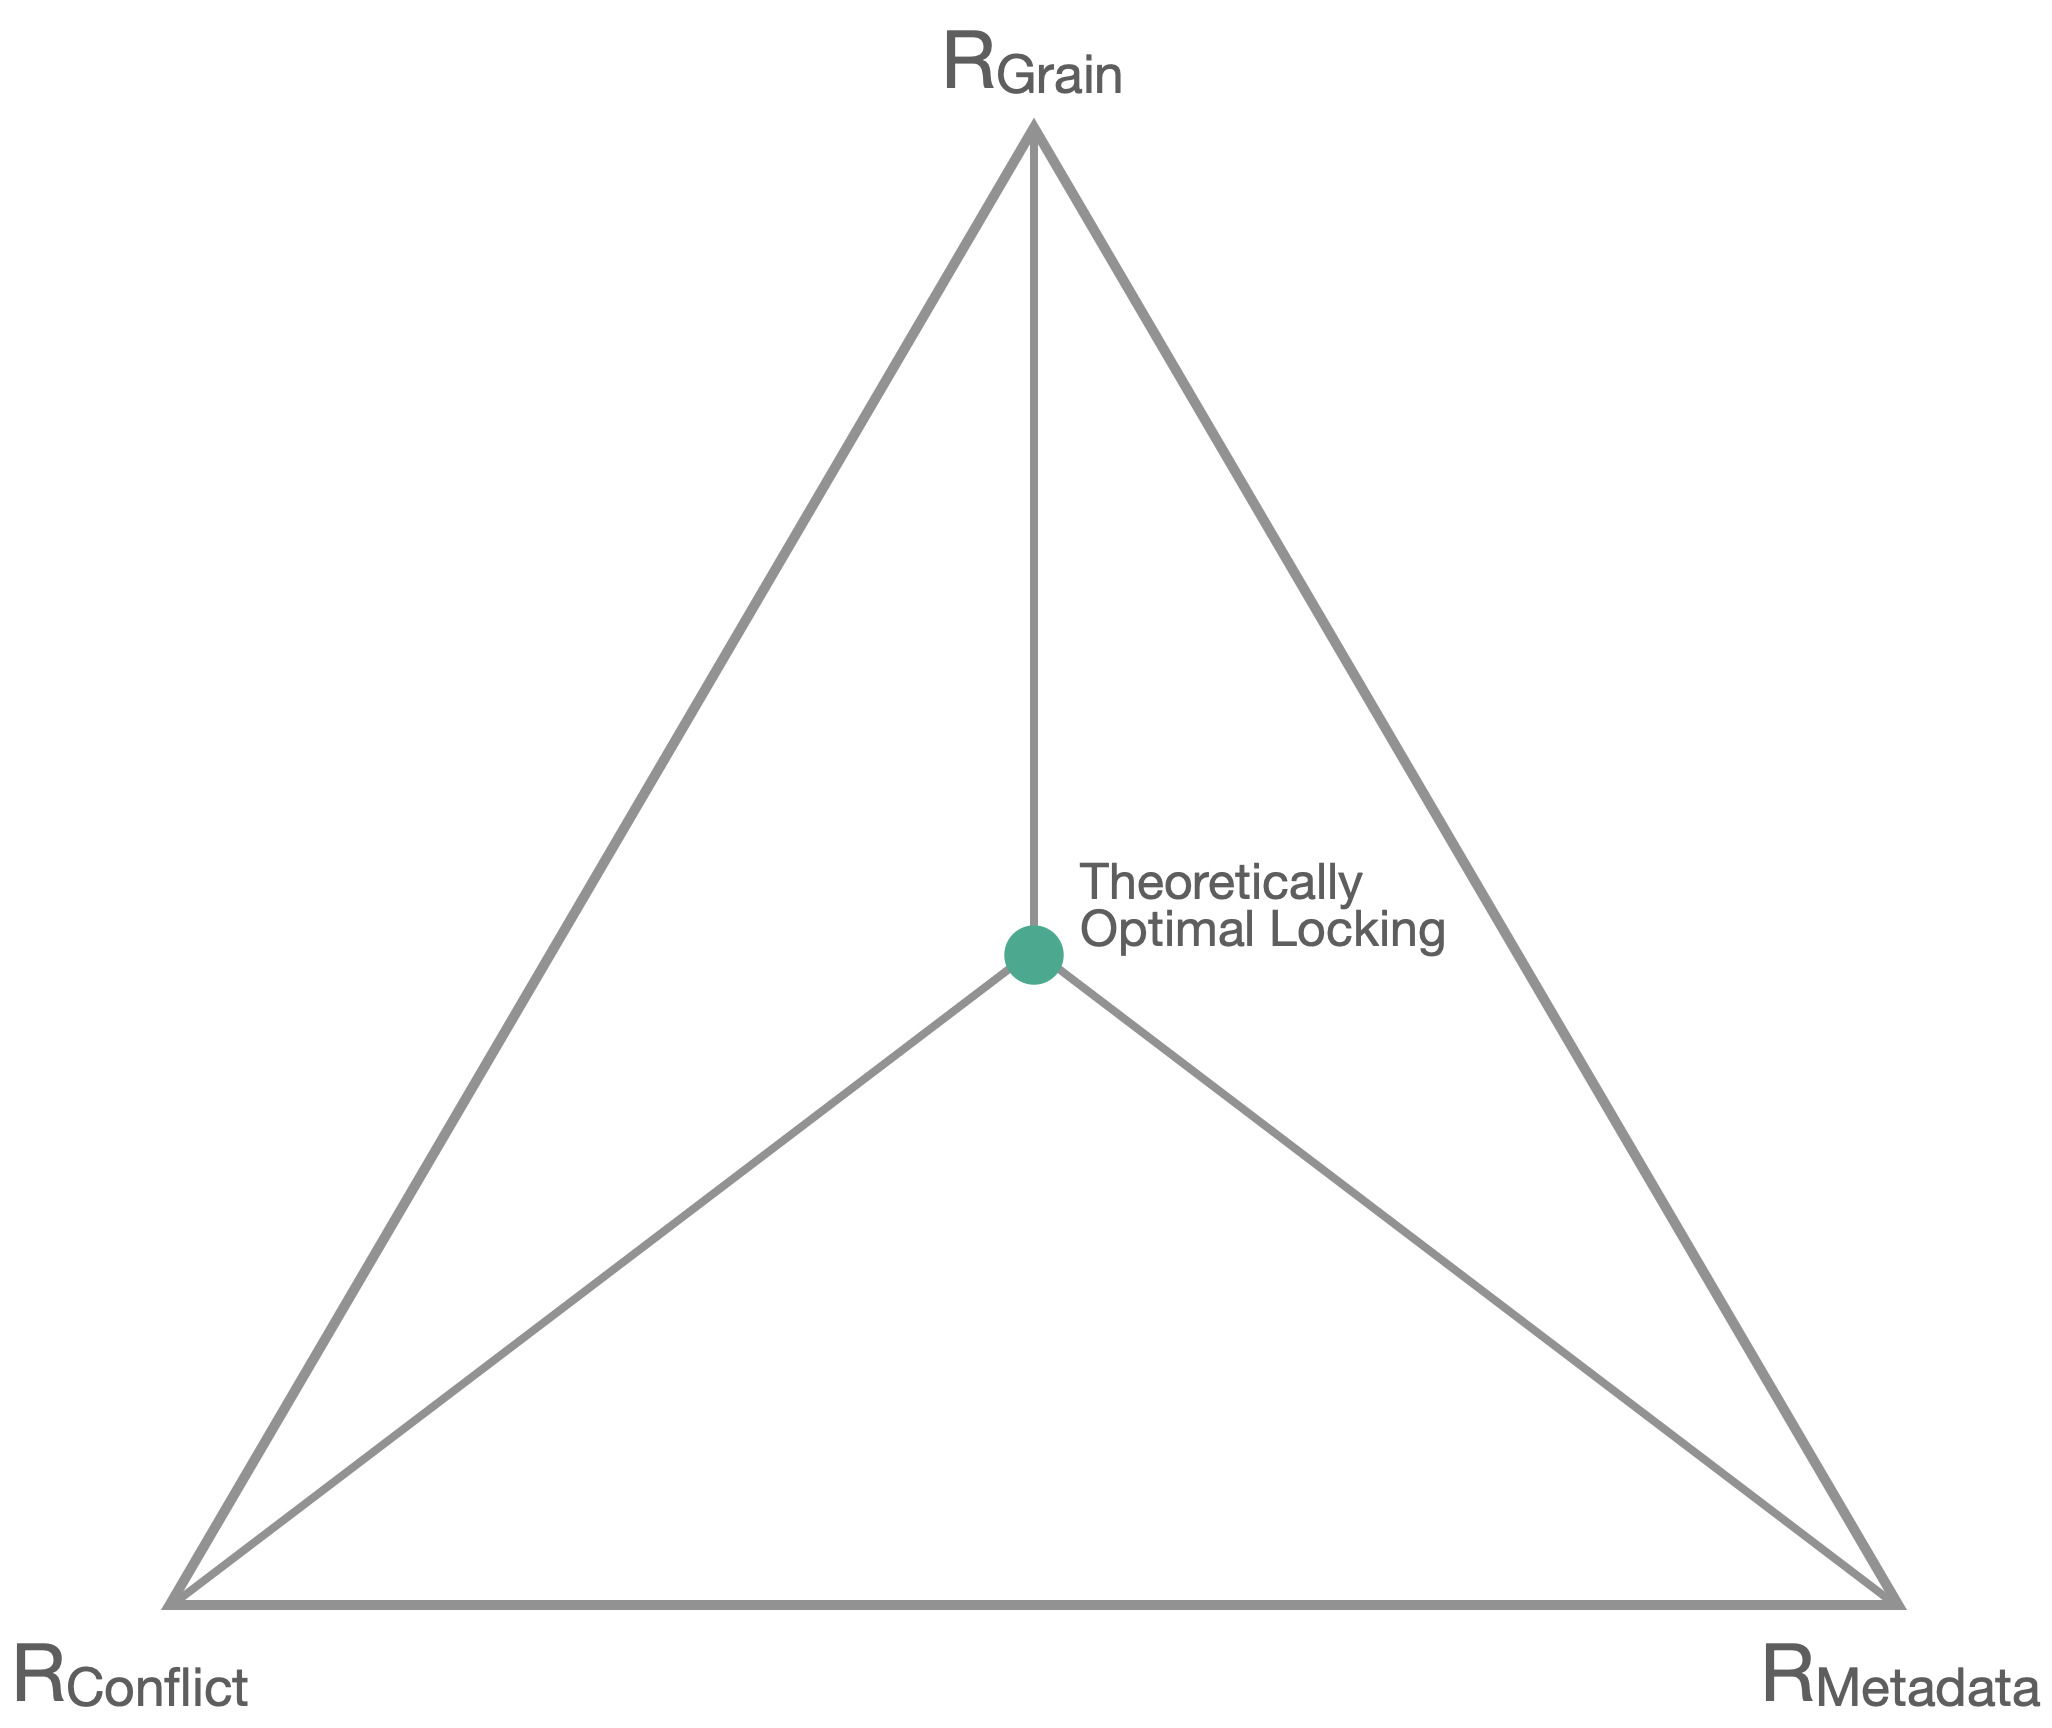
\includegraphics[width=0.8\textwidth]{figures/IdealMGLTechnique.png}
    \caption{An optimal MGL technique balances the trade-offs between the three requirements to maximize throughput.}
    \label{fig:lock_throughput}
\end{figure}

\begin{itemize}

    \item[\Rb] \emph{Finding an appropriately sized grain for a request}. When a thread requests a lock on a set of lock targets, a locking protocol must determine a lock grain for this request such that a lock on said grain maximizes throughput. This involves considering the topology of the hierarchy and the relationships between vertices to minimize grain conflicts.
    
    \item[\Rc] \emph{Efficiently detecting conflicts between locks}. Mode conflicts and grain conflicts between lock requests must be detected correctly to guarantee data consistency and efficiently to improve lock throughput. Mode conflicts can be detected by maintaining a lock table that records the lock mode for each transaction. Grain conflicts are more complex and often require sub-graph traversal to identify overlapping grains. A locking protocol must ensure that a locked grain is not accessed by a transaction with a conflicting mode. Several MGL protocols use additional metadata to optimize the detection of grain conflicts.

    \item[\Rd] \emph{Housekeeping the metadata required to implement the locking protocol.} The additional metadata required to implement the locking protocol and the conflict detection mechanism must be managed efficiently to minimize the overhead of using that particular locking protocol. If metadata management is prohibitively expensive for specific workloads, the locking protocol may not be practical for real-world applications that encounter those workloads. 

\end{itemize}


The goal of a correct MGL technique is to maximize throughput. This throughput is measured by the number of lock requests that can be granted in a unit of time. Depending on the locking protocol, this can translate to optimizing the former three requirements. For example, a locking protocol that uses a deterministic traversal to detect conflicts can detect conflicts more efficiently by implementing graph-isomorphism tests. This, in turn, increases the system's throughput but incurs a higher memory footprint. A locking protocol that uses labelling omits traversals altogether and needs to optimize the metadata management to increase throughput. 


